%++++++++++++++++++++++++++++++++++++++++s\\
\documentclass[letterpaper,12pt]{article}
\usepackage{tabularx} % extra features for tabular environment
\usepackage{amsmath}  % improve math presentation
\usepackage{graphicx} % takes care of graphic including machinery
\usepackage[margin=1in,letterpaper]{geometry} % decreases margins
\usepackage{cite} % takes care of citations
\usepackage[final]{hyperref} % adds hyper links inside the generated pdf file
\usepackage{caption}
\usepackage{float}
\usepackage{subcaption}
\usepackage{hyperref}
\hypersetup{
	colorlinks=true,       % false: boxed links; true: colored links
	linkcolor=blue,        % color of internal links
	citecolor=blue,        % color of links to bibliography
	filecolor=magenta,     % color of file links
	urlcolor=blue         
}
%++++++++++++++++++++++++++++++++++++++++


\begin{document}

\title{732A75 Advanced Data Mining laboratory 3 report}
\author{Yuki Washio and Nicolas Taba}
\date{\today}
\maketitle



\section{Introduction}

The aim of this laboratory exercise is to test the limits of the clustering algorithm using the distance metric and understand that the clsutering algorithms can sometimes fail to provide clusters that correspond to classes that we (humans) may intuit better.

In order to illustrate this, we are using the MONK1 dataset.
[Present the dataset here]. [use link that is in masters bookmarks] Illustrate with an example such as wearing a certain type of clothes and a red tie for example.

We will first start an exploratory analysis and clustering using appropriate clustering methods for our problem using the distance as a metric and trying to improve on it as much as possible before turning to assosciation analysis.


\section{Clustering}

The dataset presents categorical data. We should use hierarchical methods to create our cluster and obtain the desired 2 clusters.

We are going to use the average linkage that uses euclidean distance as a metric.

\begin{figure}[H]
\begin{subfigure}{.5\textwidth}
  \centering
  % include first image
  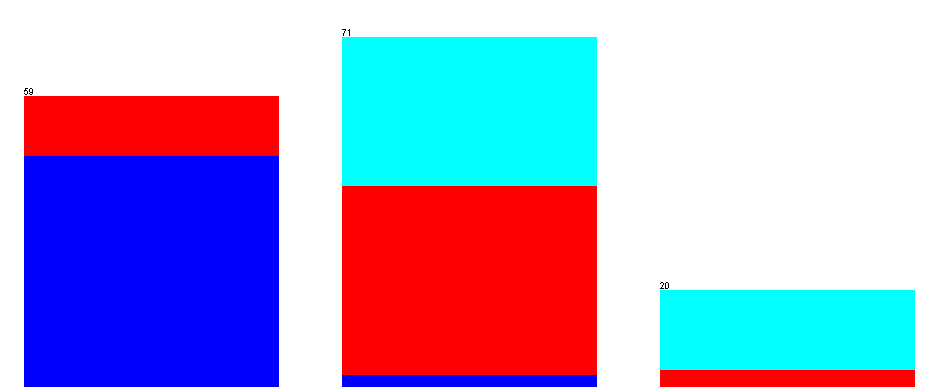
\includegraphics[width=.8\linewidth]{3bins_petalwidth}  
  \caption{data separated into 3 bins according to petalwidth}
  \label{fig:sub-first_1}
\end{subfigure}
\begin{subfigure}{.5\textwidth}
  \centering
  % include second image
  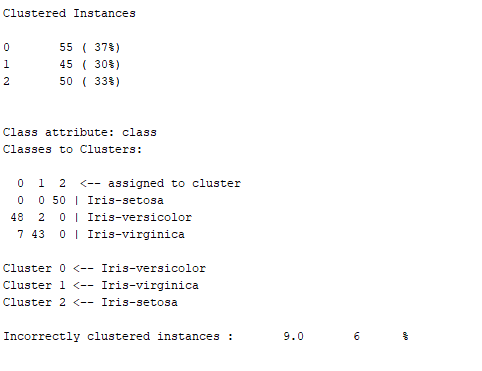
\includegraphics[width=.8\linewidth]{3bins_3cl_output}  
  \caption{kmeans clustering using k=3}
  \label{fig:sub-second_1}
\end{subfigure}
\caption{clustering using Kmeans with k=3 and n=3 bins}
\label{fig:fig_1}
\end{figure}

The algorithm does not perform well and guesses incorrectly about half of the time. This is not a satisfactory result. [exploration of the data by looking at a particular attribute].

Find a way to improve the classification by adding an outlier cluster.



\begin{figure}[H] 
  \centering
      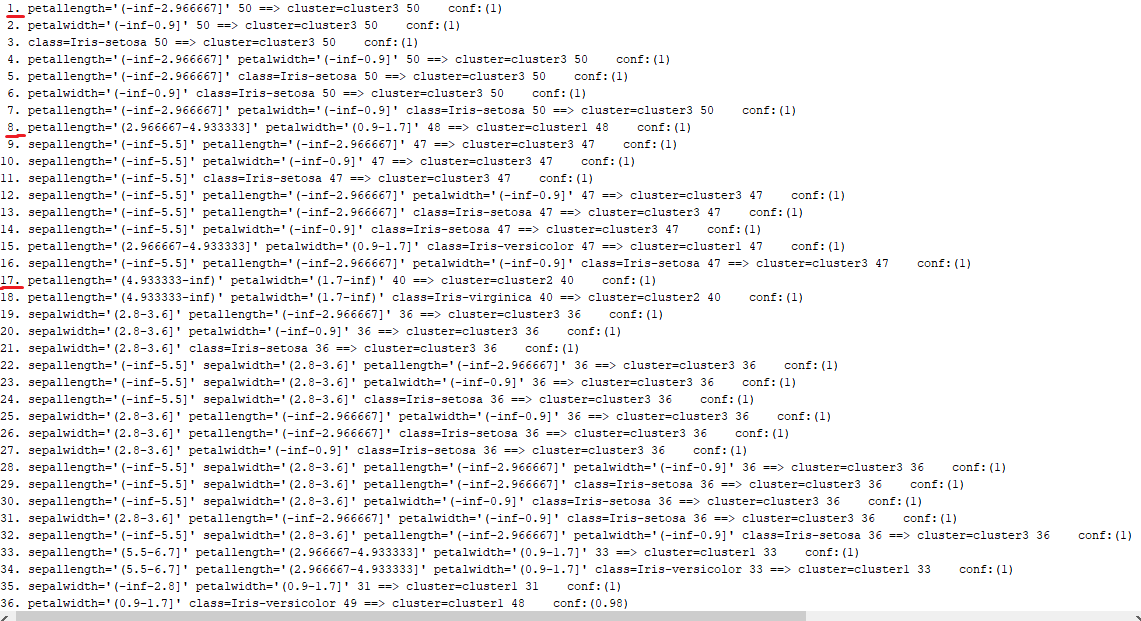
\includegraphics[width=0.8\columnwidth]{3_bins_3cl_apriori_rules}
        \caption{
                \label{fig:3bins_3cl_apriori}  
                Apriori rules for k=3 and n=3 bins.
        }
\end{figure}



\section{Assosciation analysis}


look at the rules of the problem that we want to solve and find them in there



\section{Discussion}



\end{document}
